\section{Machine Learning}

\begin{itemize}
\item What is machine learning?

\item Why is it useful for HEP? (Problems are multivariate...)

\item Supervised learning, i.e.\ have labelled data.

\item Binary classification tasks: Every training example has a label indicating
  the class membership.

\item In HEP, the positive class is typically referred to as \emph{signal} while
  the negative class is referred to as \emph{background}.

\item What is training data, etc.

\item What is training.
\end{itemize}


\subsection{Boosted Decision Trees}

Boosted decision trees (BDT) are classification and regression algorithms
composed of multiple \emph{decision trees}. This ensemble of decision trees is
created using an algorithm referred to as \emph{boosting}, which iteratively
fits shallow decision trees--or in general, any \emph{weak learning
  algorithm}--to altered versions of the training data. The training data is
modified at every iteration to emphasise errors made in previous
iterations. Finally, the predictions of the ensemble of trees are combined with
the goal of providing superior classification/regression performance compared to
a single decision tree. In the following a description of the BDT algorithm
implemented in \textsc{TMVA}~\cite{TMVA} is given, which is later used in the
search for Higgs boson pair production.


\subsubsection{Classification and Regression Trees}

Classification and regression trees~\cite{Breiman:1984jka,hastie09}, hereafter
collectively referred to as \emph{decision trees}, are used as the basis for
BDT. A decision tree partitions an $n$-dimensional space with coordinates
$\myvec{x} = (x_1, \dots, x_n)$ by recursively performing binary splits along
the coordinate axes until a stopping criterion is met. The resulting binary tree
structure and partitioning is illustrated in \Cref{fig:decision_tree} for a
two-dimensional example. A decision tree with $J$~leaf nodes partitions the
input space into $J$~mutually disjoint subregions denoted by $R_j$ for
$j = 1, \dots, J$. A constant value $c_j$ is assigned to every region $R_j$ such
that the prediction of a decision tree for a point~$\myvec{x}$ can expressed as
\begin{align*}
  h\bigl( \myvec{x}; \{c_j, R_j\}_{j=1}^{J} \bigr) = \sum_{j = 1}^{J} c_j \, \mathbf{1}(\myvec{x} \in R_j) \qquad \text{with} \qquad \mathbf{1}(\myvec{x} \in R_j) =
  \begin{cases}
    1, & \myvec{x} \in R_j \\
    0, & \text{else}
  \end{cases} \,\text{,}
\end{align*}
where $\{c_j, R_j\}_{j=1}^{J}$ represents the parameters that specify the
decision tree~\cite{hastie09}.

\begin{figure}[htbp]
  \centering

  \begin{subfigure}[b]{0.46\textwidth}
    \centering
    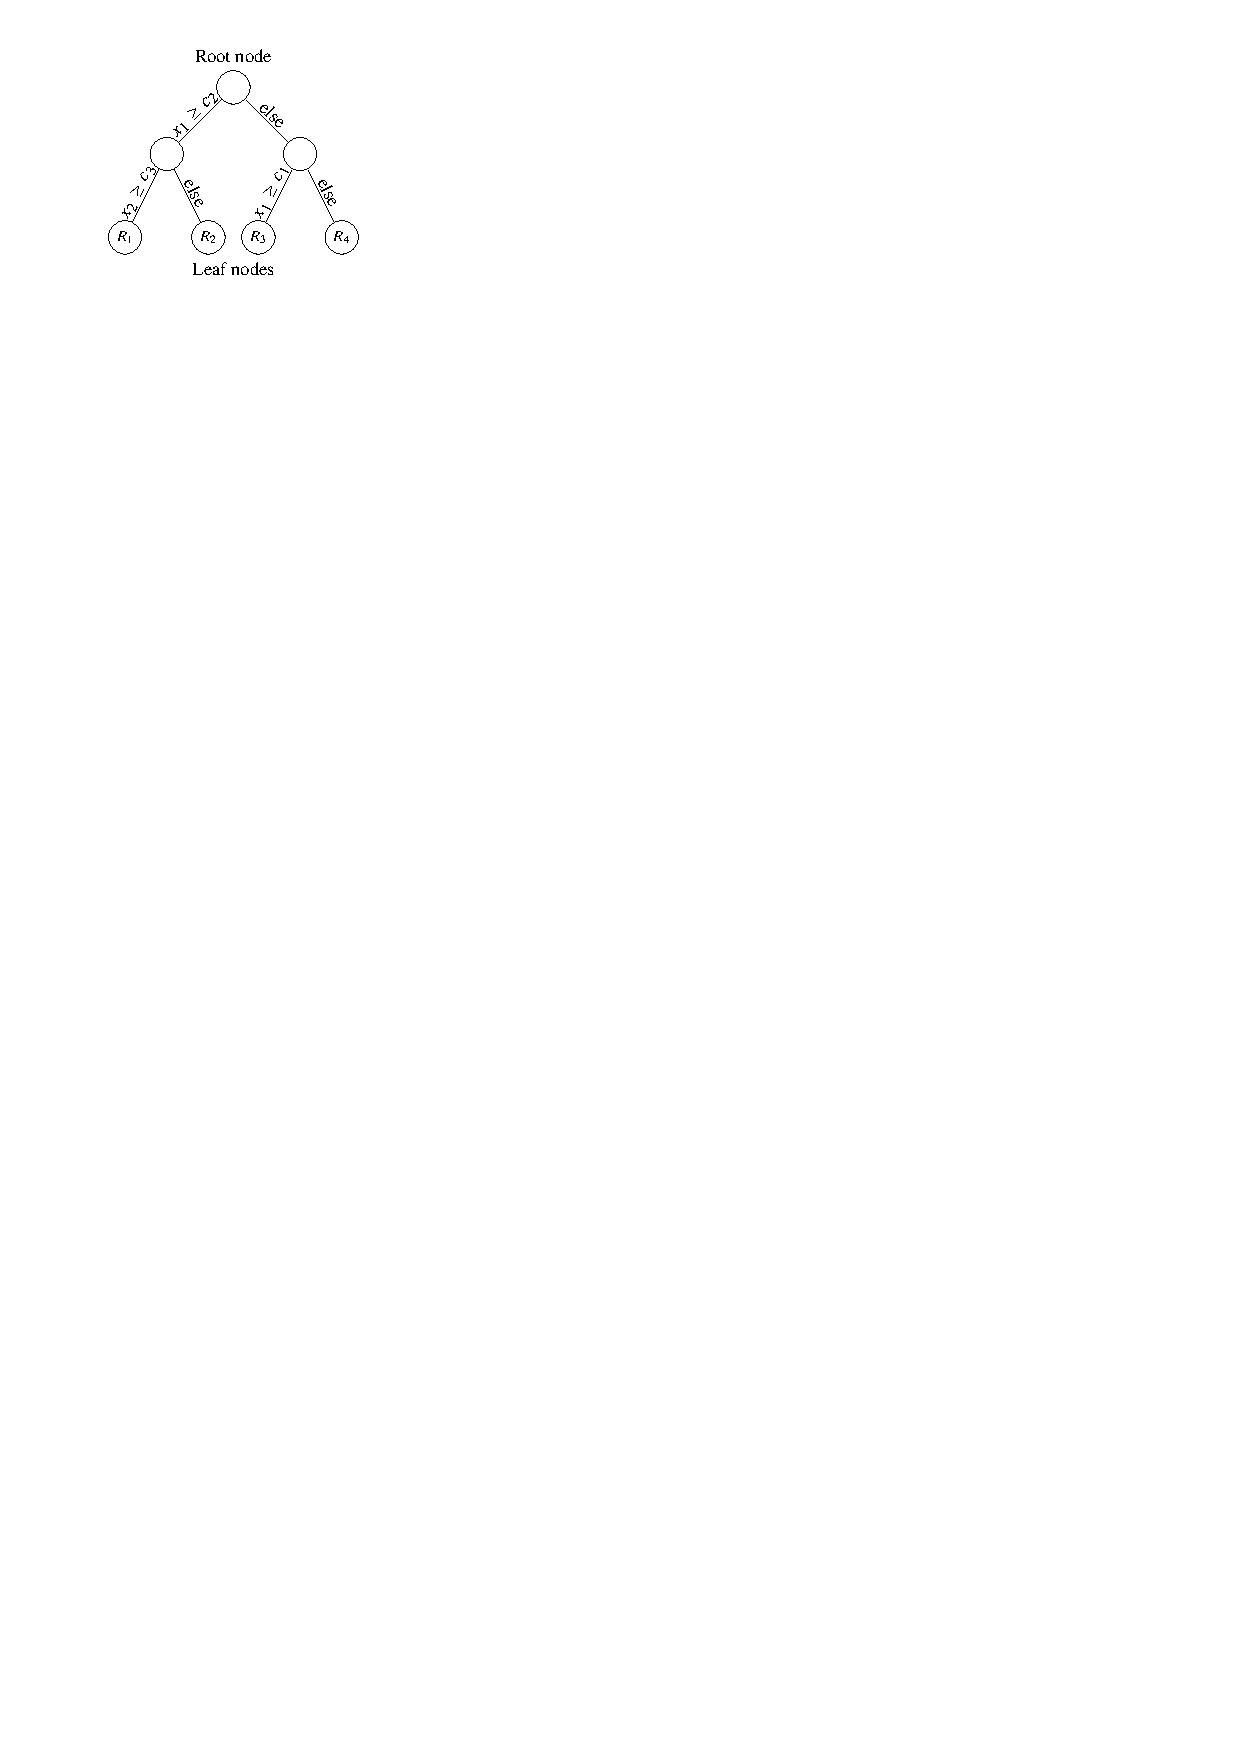
\includegraphics[scale=1.05]{ml/decision_tree}
    \caption{Binary tree structure of a decision tree.}
  \end{subfigure}\hfill%
  \begin{subfigure}[b]{0.46\textwidth}
    \centering
    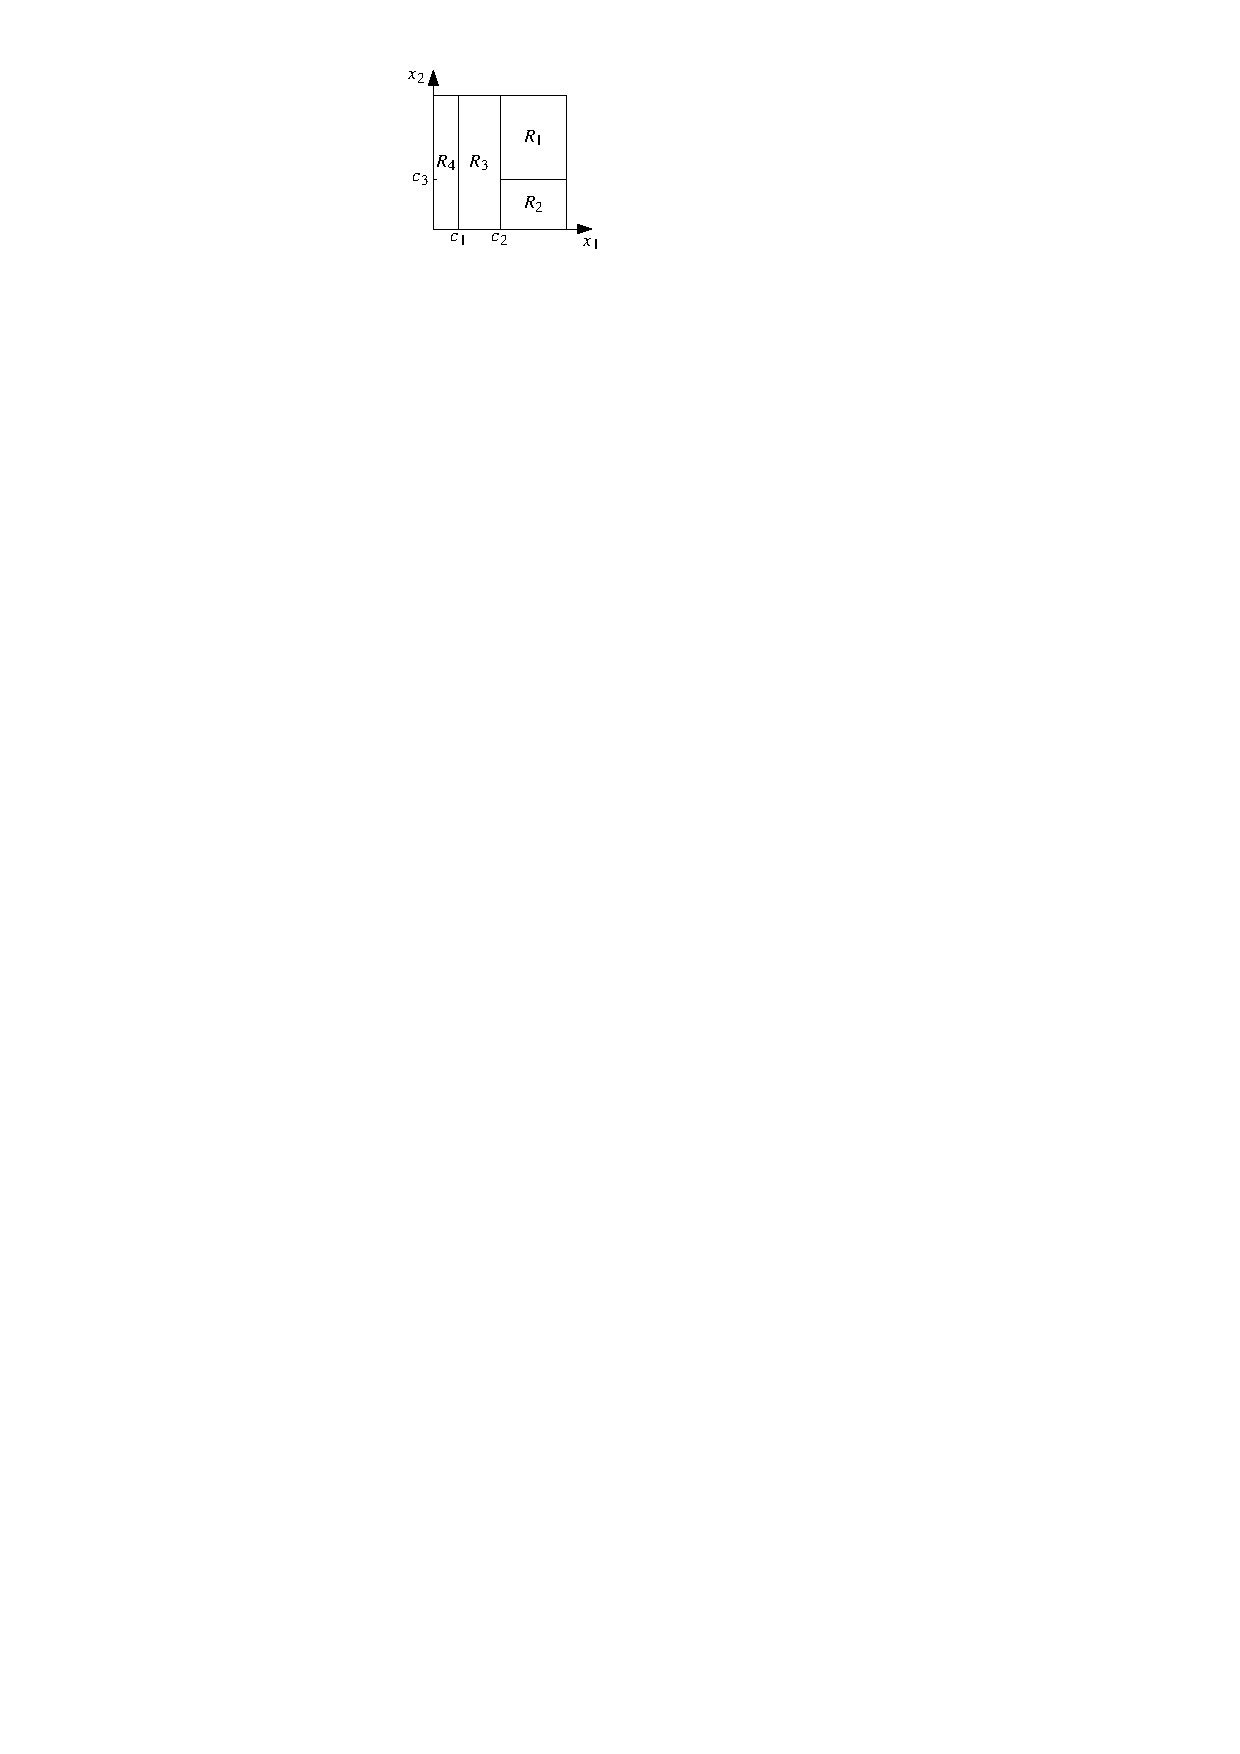
\includegraphics[scale=1.05]{ml/decision_tree_partitioning}
    \vspace*{0.7em}
    \caption{Partitioning resulting from the binary tree in (a).}
  \end{subfigure}\hfill%

  \caption{Example of a decision tree operating on a two-dimensional space with
    coordinates $\myvec{x} = (x_1, x_2)$. The tree has a depth of two and four
    leaf nodes that define the regions $R_1, \dots, R_4$. The figure is adapted
    from Ref.~\cite{hastie09}.}%
  \label{fig:decision_tree}
\end{figure}

Classification trees are constructed with the goal that the partitioning of the
input space yields subregions with low impurity, that is, the regions are mostly
populated by training examples of a single class. In this case, the impurity of
a tree node is quantified by the Gini index
\begin{align*}
  I_{\text{G}}(p) = 2 p (1 - p) \,\text{,}
\end{align*}
where $p$ is the proportion of examples from the positive class in a given
node~\cite{hastie09}. A \emph{greedy} strategy is adopted to grow decision trees
by performing the best possible split at every node. This split is determined by
minimising the weighted sum of Gini impurities of the resulting daughter nodes,
where impurities are weighted according to the total weight of training examples
populating a given node. In the classification case, the constants $c_j$
assigned to leaf nodes of the tree are either--depending on the algorithm
configuration--the proportion of examples from the positive class or the class
label of the majority class in a given leaf node.

Regression trees are constructed using a similar approach, however, with an
altered splitting criterion and different assigment of constants to leaf
nodes. Consider the split of a parent node into a left (L) and right (R)
daughter node. Let $(y, w)$ denote the tuple of regression target and weight of
a given training example. Moreover, let $T_{\text{L}}$ and $T_{\text{R}}$ denote
the set of $(y, w)$ for training examples populating the left and right daughter
node, respectively. The constants $c_{\text{L}}$ and $c_{\text{R}}$ assigned to
the daughter nodes are given by
\begin{align*}
  c_{\text{L}} = \frac{\sum_{(y, w) \in T_{\text{L}}} w y}{\sum_{(y, w) \in T_{\text{L}}} w} \qquad \text{and} \qquad c_{\text{R}} = \frac{\sum_{(y, w) \in T_{\text{R}}} w y}{\sum_{(y, w) \in T_{\text{R}}} w} \,\text{,}
\end{align*}
which is the weighted mean of the regression target for the training examples
populating the left and right node, respectively. The best possible split of a
node in a regression tree is chosen such that the squared error defined as
\begin{align*}
  \sum_{(y, w) \in T_{\text{L}}} w (y - c_{\text{L}})^2 + \sum_{(y, w) \in T_{\text{R}} } w (y - c_{\text{R}})^2
\end{align*}
is minimised.


\subsubsection{Boosting of Decision Trees}

Boosting is an approach of solving a prediction problem by constructing an
additive model of the form
\begin{align*}
  F_{M}\bigl(\myvec{x}; \{ \beta_m, \gamma_{m} \}_{m=1}^{M} \bigr) = \sum_{m = 1}^{M} \beta_m b(\myvec{x}; \gamma_{m}) \,\text{,}
\end{align*}
where $\beta_m$ are coefficients and $b(\myvec{x}; \gamma_{m})$ are basis
functions parameterised
by~$\gamma_{m}$~\cite{Friedman:2000,Friedman:2001wbq}. While there is some
flexibility in choosing the family of basis functions, boosting is frequently
performed using classification or regression trees, which will be the subject of
the remainder of this section. Given a sample of training data, boosting fits an
additive model in a \emph{forward stagewise fashion}, which refers to an
iterative procedure in which the $m$-th stage of the model given by
\begin{align*}
  F_{m}\bigl(\myvec{x}; \{ \beta_{n}, \gamma_{n} \}_{n=1}^{m} \bigr) = F_{m - 1}\bigl( \myvec{x}; \{ \beta_{n}, \gamma_{n} \}_{n=1}^{m-1} \bigr) + \beta_m b(\myvec{x}; \gamma_{m})
\end{align*}
is determined by optimising an objective function with respect to $\beta_{m}$
and $\gamma_{m}$ while leaving the other parameters unchanged~\cite{hastie09}. A
number of boosting algorithms exist, among the most prevalent ones being
\textsc{AdaBoost}~\cite{freund_shapire:adaboost,freund_shapire:adaboost2} and
\emph{gradient boosting}~\cite{Friedman:2001wbq}. Gradient boosting provides a
framework for constructing additive models that minimise an arbitrary
differentiable loss function. As a result, gradient boosting is highly
versatile, allowing to solve numerous prediction problems that can be expressed
as the minimisation of a loss function.


Consider a binary classification problem with predictors $\myvec{X}$ and class
labels $Y$, which are taken to be $Y = +1$ for the positive and $Y = -1$ for the
negative class. Both $\myvec{X}$ and $Y$ are considered to be random
variables. Further, let
\begin{align}
  L(Y, F(\myvec{X})) = \log\mathopen{}\left(
  1 + e^{-Y F(\myvec{X})}
  \right)\mathclose{}
  \label{eq:loss_gradboost}
\end{align}
be a loss function and $F$~a function of the predictors. The function $F^*$ that
minimises the expected loss is given by
\begin{align}
  F^*(\myvec{x})
  = \argmin_F \, \expect[ L(Y, F) \mid \myvec{X} = \myvec{x} ]
  = \log\mathopen{}\left(
  \frac{
  \mathbb{P}(Y = +1 \mid \myvec{X} = \myvec{x})
  }{
  \mathbb{P}(Y = -1 \mid \myvec{X} = \myvec{x})
  }
  \right)\mathclose{} \,\text{,}
  \label{eq:gradboost_logodds}
\end{align}
which are the log-odds of an observation with predictors~$\myvec{x}$ belonging
to the positive class, thus motivating the choice of loss function in
\Cref{eq:loss_gradboost} for classification.
% \footnote{Noting that
%   \begin{align*}
%     \mathbb{P}(Y = +1 \mid \myvec{X} = \myvec{x}) = \frac{1}{1 + \exp(-F^*(\myvec{x}))} \qquad \mathbb{P}(Y = -1 \mid \myvec{X} = \myvec{x}) = \frac{1}{1 + \exp(+F^*(\myvec{x}))} \,\text{,}
%   \end{align*}
%   the loss function of \Cref{eq:loss_gradboost} follows from the binary
%   cross-entropy (BCE)
%   \begin{align*}
%     L_{\text{BCE}} =
%     \begin{cases}
%       - \log\mathbb{P}(Y = +1 \mid \myvec{X}), & Y = +1 \\
%       - \log\mathbb{P}(Y = -1 \mid \myvec{X}), & Y = -1
%     \end{cases}
%     \,\text{,}
%   \end{align*}
%   further motivating the use of this particular loss function and making a
%   connection to the classification approach using neural networks that will be
%   discussed in~\Cref{sec:neural_networks}.}
Gradient boosting with decision trees can be used to find an approximation to
$F^*$ using finite samples of training data.

In the following, the \textsc{TreeBoost} algorithm~\cite{Friedman:2001wbq} for
binary classification is outlined. This algorithm is employed by
\textsc{TMVA}~\cite{TMVA} for gradient boosting with decision trees. The
description is based on Ref.~\cite{Friedman:2001wbq} with few modifications, the
most significant one being the incorporation of sample weights for the training
examples.
\begin{enumerate}
  \setlength{\itemsep}{4pt}

\item Initialise $F_0(\myvec{x}) = 0$

\item For $m = 1$ to $M$ (boosting iterations):
  \begin{enumerate}
    \setlength{\itemsep}{4pt}

  \item Calculate the pseudoresiduals
    \begin{align*}
      r_i
      = - \left. \frac{\partial L(y_i, F(\myvec{x}_i))}{\partial F(\myvec{x}_i)}\right|_{F(\myvec{x}_i) = F_{m - 1}(\myvec{x}_i)}
      \overset{\text{Eq.\ (\ref{eq:loss_gradboost})}}{=} \frac{y_i}{1 + \exp(y_i F_{m-1}(\myvec{x}_i))}
    \end{align*}
    for all training examples, where $\myvec{x}_i$ are the predictors and $y_i$
    the class label of the $i$-th training example, respectively.

  \item Using the training data, fit a regression tree to estimate the
    pseudoresiduals given the predictors~$\myvec{x}$. The prediction of the
    $m$-th regression tree is denoted by
    $h\bigl( \myvec{x}; \{c_{jm}, R_{jm}\}_{j=1}^{J_{m}} \bigr)$, where $J_{m}$
    is the number of leaf nodes, $c_{jm}$ is the constant predicted by the
    $j$-th leaf node, and $R_{jm}$ is the region defined by the $j$-th leaf
    node.

  \item The leaf node constants of the regression tree,
    $\{c_{jm}\}_{j=1}^{J_{m}}$, are updated to minimise
    \begin{align*}
      \sum_i w_i \cdot
      L\mathopen{}\left( y_i, F_{m - 1}(\myvec{x}_i)
      + h\bigl( \myvec{x}_i; \{c_{jm}, R_{jm}\}_{j=1}^{J_{m}} \bigr)
      \right)\mathclose{}
      \,\text{,}
    \end{align*}
    where $w_i$ is the weight of training example $i$ and the sum goes over all
    training examples. This is equivalent to minimising the weighted mean of the
    loss for the current boosting iteration. This optimisation problem has no
    analytical minimiser. Instead, the $\{c_{jm}\}_{j=1}^{J_{m}}$ are chosen to
    approximately minimise the above criterion by performing a single step of
    Newton's method.\footnote{The starting point for Newton's method is taken to
      be $c_{jm} = 0$ for all leaf nodes.} For the loss function in
    \Cref{eq:loss_gradboost}, this yields updated leaf node constants
    \begin{align*}
      c_{jm}^\prime = \frac{ \sum_i w_i r_i }{ \sum_i w_i |r_i| (1 - |r_i|)} \,\text{,}
    \end{align*}
    where the sum goes over the training examples populating the $j$-th leaf of
    the tree. This step is specific to the \textsc{TreeBoost} algorithm proposed
    by Friedman.

  \item Perform a gradient descent step by setting
    \begin{align*}
      F_m(x) = F_{m - 1}(x) + \nu \cdot h\bigl( \myvec{x}; \{c_{jm}^\prime, R_{jm}\}_{j=1}^{J_{m}} \bigr) \,\text{,}
    \end{align*}
    where $0 < \nu \leq 1$ is a hyperparameter of the algorithm referred to as
    the \emph{shrinkage} or \emph{learning rate}.
  \end{enumerate}

\item The final prediction of the boosting procedure, $F_{M}(x)$, can be used to
  estimate the probability $\mathbb{P}(Y = +1 \mid \myvec{X} = \myvec{x})$
  according to
  \begin{align*}
    \hat{p}(\myvec{x}) = \frac{1}{1 + \exp(-F_{M}(\myvec{x}))} \,\text{,}
  \end{align*}
  which follows from \Cref{eq:gradboost_logodds}. In HEP, this quantity is
  commonly referred to as the \emph{BDT score}.

\end{enumerate}

Gradient descent in function space...


\subsection{Neural Networks}%
\label{sec:neural_networks}

\subsubsection{Recurrent Neural Networks}%
\label{sec:rnn}


%%% Local Variables:
%%% mode: latex
%%% TeX-master: "../../phd_thesis"
%%% End:
